\documentclass[12pt,twoside]{article}

\newcommand{\reporttitle}{Project 1: Navigation}
\newcommand{\reportauthor}{Thomas Teh}
\newcommand{\reporttype}{Project Report}
\newcommand{\cid}{0124 3008}

% include files that load packages and define macros
%%%%%%%%%%%%%%%%%%%%%%%%%%%%%%%%%%%%%%%%%
% University Assignment Title Page 
% LaTeX Template
% Version 1.0 (27/12/12)
%
% This template has been downloaded from:
% http://www.LaTeXTemplates.com
%
% Original author:
% WikiBooks (http://en.wikibooks.org/wiki/LaTeX/Title_Creation)
%
% License:
% CC BY-NC-SA 3.0 (http://creativecommons.org/licenses/by-nc-sa/3.0/)
% 
% Instructions for using this template:
% This title page is capable of being compiled as is. This is not useful for 
% including it in another document. To do this, you have two options: 
%
% 1) Copy/paste everything between \begin{document} and \end{document} 
% starting at \begin{titlepage} and paste this into another LaTeX file where you 
% want your title page.
% OR
% 2) Remove everything outside the \begin{titlepage} and \end{titlepage} and 
% move this file to the same directory as the LaTeX file you wish to add it to. 
% Then add \input{./title_page_1.tex} to your LaTeX file where you want your
% title page.
%
%----------------------------------------------------------------------------------------
%	PACKAGES AND OTHER DOCUMENT CONFIGURATIONS
%----------------------------------------------------------------------------------------
\usepackage{ifxetex}
\usepackage{textpos}
%\usepackage{natbib}
%\usepackage{breqn}
\usepackage{kpfonts}
\usepackage[a4paper,hmargin=2.8cm,vmargin=2.0cm,includeheadfoot]{geometry}
\usepackage{ifxetex}
\usepackage{stackengine}
\usepackage{tabularx,longtable,multirow,subfigure,caption}%hangcaption
\usepackage{fncylab} %formatting of labels
\usepackage{fancyhdr}
\usepackage{color}
\usepackage[tight,ugly]{units}
\usepackage{url}
\usepackage{float}
\usepackage[english]{babel}
\usepackage{amsmath}
\usepackage{graphicx}
\usepackage[colorinlistoftodos]{todonotes}
\usepackage{dsfont}
\usepackage{epstopdf} % automatically replace .eps with .pdf in graphics
\usepackage{natbib}
\usepackage{backref}
\usepackage{array}
\usepackage{latexsym}
\usepackage{etoolbox}
\usepackage{algorithmic}
\usepackage[]{algorithm2e}

\usepackage{enumerate} % for numbering with [a)] format 



\ifxetex
\usepackage{fontspec}
\setmainfont[Scale=.8]{OpenDyslexic-Regular}
\else
\usepackage[pdftex,pagebackref,hypertexnames=false,colorlinks]{hyperref} % provide links in pdf
\hypersetup{pdftitle={},
  pdfsubject={}, 
  pdfauthor={\reportauthor},
  pdfkeywords={}, 
  pdfstartview=FitH,
  pdfpagemode={UseOutlines},% None, FullScreen, UseOutlines
  bookmarksnumbered=true, bookmarksopen=true, colorlinks,
    citecolor=black,%
    filecolor=black,%
    linkcolor=black,%
    urlcolor=black}
\usepackage[all]{hypcap}
\fi

\usepackage{tcolorbox}

% various theorems
\usepackage{ntheorem}
\theoremstyle{break}
\newtheorem{lemma}{Lemma}
\newtheorem{theorem}{Theorem}
\newtheorem{remark}{Remark}
\newtheorem{definition}{Definition}
\newtheorem{proof}{Proof}

% example-environment
\newenvironment{example}[1][]
{ 
\vspace{4mm}
\noindent\makebox[\linewidth]{\rule{\hsize}{1.5pt}}
\textbf{Example #1}\\
}
{ 
\noindent\newline\makebox[\linewidth]{\rule{\hsize}{1.0pt}}
}



%\renewcommand{\rmdefault}{pplx} % Palatino
% \renewcommand{\rmdefault}{put} % Utopia

\ifxetex
\else
\renewcommand*{\rmdefault}{bch} % Charter
\renewcommand*{\ttdefault}{cmtt} % Computer Modern Typewriter
%\renewcommand*{\rmdefault}{phv} % Helvetica
%\renewcommand*{\rmdefault}{iwona} % Avant Garde
\fi

\setlength{\parindent}{0em}  % indentation of paragraph

\setlength{\headheight}{14.5pt}
\pagestyle{fancy}
\fancyfoot[ER,OL]{\thepage}%Page no. in the left on
                                %odd pages and on right on even pages
\fancyfoot[OC,EC]{\sffamily }
\renewcommand{\headrulewidth}{0.1pt}
\renewcommand{\footrulewidth}{0.1pt}
\captionsetup{margin=10pt,font=small,labelfont=bf}


%--- chapter heading

\def\@makechapterhead#1{%
  \vspace*{10\p@}%
  {\parindent \z@ \raggedright %\sffamily
        %{\Large \MakeUppercase{\@chapapp} \space \thechapter}
        %\\
        %\hrulefill
        %\par\nobreak
        %\vskip 10\p@
    \interlinepenalty\@M
    \Huge \bfseries 
    \thechapter \space\space #1\par\nobreak
    \vskip 30\p@
  }}

%---chapter heading for \chapter*  
\def\@makeschapterhead#1{%
  \vspace*{10\p@}%
  {\parindent \z@ \raggedright
    \sffamily
    \interlinepenalty\@M
    \Huge \bfseries  
    #1\par\nobreak
    \vskip 30\p@
  }}
  



% %%%%%%%%%%%%% boxit
\def\Beginboxit
   {\par
    \vbox\bgroup
	   \hrule
	   \hbox\bgroup
		  \vrule \kern1.2pt %
		  \vbox\bgroup\kern1.2pt
   }

\def\Endboxit{%
			      \kern1.2pt
		       \egroup
		  \kern1.2pt\vrule
		\egroup
	   \hrule
	 \egroup
   }	

\newenvironment{boxit}{\Beginboxit}{\Endboxit}
\newenvironment{boxit*}{\Beginboxit\hbox to\hsize{}}{\Endboxit}



\allowdisplaybreaks

\makeatletter
\newcounter{elimination@steps}
\newcolumntype{R}[1]{>{\raggedleft\arraybackslash$}p{#1}<{$}}
\def\elimination@num@rights{}
\def\elimination@num@variables{}
\def\elimination@col@width{}
\newenvironment{elimination}[4][0]
{
    \setcounter{elimination@steps}{0}
    \def\elimination@num@rights{#1}
    \def\elimination@num@variables{#2}
    \def\elimination@col@width{#3}
    \renewcommand{\arraystretch}{#4}
    \start@align\@ne\st@rredtrue\m@ne
}
{
    \endalign
    \ignorespacesafterend
}
\newcommand{\eliminationstep}[2]
{
    \ifnum\value{elimination@steps}>0\leadsto\quad\fi
    \left[
        \ifnum\elimination@num@rights>0
            \begin{array}
            {@{}*{\elimination@num@variables}{R{\elimination@col@width}}
            |@{}*{\elimination@num@rights}{R{\elimination@col@width}}}
        \else
            \begin{array}
            {@{}*{\elimination@num@variables}{R{\elimination@col@width}}}
        \fi
            #1
        \end{array}
    \right]
    & 
    \begin{array}{l}
        #2
    \end{array}
    &%                                    moved second & here
    \addtocounter{elimination@steps}{1}
}
\makeatother

%% Fast macro for column vectors
\makeatletter  
\def\colvec#1{\expandafter\colvec@i#1,,,,,,,,,\@nil}
\def\colvec@i#1,#2,#3,#4,#5,#6,#7,#8,#9\@nil{% 
  \ifx$#2$ \begin{bmatrix}#1\end{bmatrix} \else
    \ifx$#3$ \begin{bmatrix}#1\\#2\end{bmatrix} \else
      \ifx$#4$ \begin{bmatrix}#1\\#2\\#3\end{bmatrix}\else
        \ifx$#5$ \begin{bmatrix}#1\\#2\\#3\\#4\end{bmatrix}\else
          \ifx$#6$ \begin{bmatrix}#1\\#2\\#3\\#4\\#5\end{bmatrix}\else
            \ifx$#7$ \begin{bmatrix}#1\\#2\\#3\\#4\\#5\\#6\end{bmatrix}\else
              \ifx$#8$ \begin{bmatrix}#1\\#2\\#3\\#4\\#5\\#6\\#7\end{bmatrix}\else
                 \PackageError{Column Vector}{The vector you tried to write is too big, use bmatrix instead}{Try using the bmatrix environment}
              \fi
            \fi
          \fi
        \fi
      \fi
    \fi
  \fi 
}  
\makeatother

\robustify{\colvec}

%%% Local Variables: 
%%% mode: latex
%%% TeX-master: "notes"
%%% End: 
 % various packages needed for maths etc.
% quick way of adding a figure
\newcommand{\fig}[3]{
 \begin{center}
 \scalebox{#3}{\includegraphics[#2]{#1}}
 \end{center}
}

%\newcommand*{\point}[1]{\vec{\mkern0mu#1}}
\newcommand{\ci}[0]{\perp\!\!\!\!\!\perp} % conditional independence
\newcommand{\point}[1]{{#1}} % points 
\renewcommand{\vec}[1]{{\boldsymbol{{#1}}}} % vector
\newcommand{\mat}[1]{{\boldsymbol{{#1}}}} % matrix
\newcommand{\R}[0]{\mathds{R}} % real numbers
\newcommand{\Z}[0]{\mathds{Z}} % integers
\newcommand{\N}[0]{\mathds{N}} % natural numbers
\newcommand{\nat}[0]{\mathds{N}} % natural numbers
\newcommand{\Q}[0]{\mathds{Q}} % rational numbers
\ifxetex
\newcommand{\C}[0]{\mathds{C}} % complex numbers
\else
\newcommand{\C}[0]{\mathds{C}} % complex numbers
\fi
\newcommand{\tr}[0]{\text{tr}} % trace
\renewcommand{\d}[0]{\mathrm{d}} % total derivative
\newcommand{\inv}{^{-1}} % inverse
\newcommand{\id}{\mathrm{id}} % identity mapping
\renewcommand{\dim}{\mathrm{dim}} % dimension
\newcommand{\rank}[0]{\mathrm{rk}} % rank
\newcommand{\determ}[1]{\mathrm{det}(#1)} % determinant
\newcommand{\scp}[2]{\langle #1 , #2 \rangle}
\newcommand{\kernel}[0]{\mathrm{ker}} % kernel/nullspace
\newcommand{\img}[0]{\mathrm{Im}} % image
\newcommand{\idx}[1]{{(#1)}}
\DeclareMathOperator*{\diag}{diag}
\newcommand{\E}{\mathds{E}} % expectation
\newcommand{\var}{\mathds{V}} % variance
\newcommand{\gauss}[2]{\mathcal{N}\big(#1,\,#2\big)} % gaussian distribution N(.,.)
\newcommand{\gaussx}[3]{\mathcal{N}\big(#1\,|\,#2,\,#3\big)} % gaussian distribution N(.|.,.)
\newcommand{\gaussBig}[2]{\mathcal{N}\left(#1,\,#2\right)} % see above, but with brackets that adjust to the height of the arguments
\newcommand{\gaussxBig}[3]{\mathcal{N}\left(#1\,|\,#2,\,#3\right)} % see above, but with brackets that adjust to the height of the arguments
\DeclareMathOperator{\cov}{Cov} % covariance (matrix) 
\ifxetex
\renewcommand{\T}[0]{^\top} % transpose
\else
\newcommand{\T}[0]{^\top}
\fi
% matrix determinant
\newcommand{\matdet}[1]{
\left|
\begin{matrix}
#1
\end{matrix}
\right|
}



%%% various color definitions
\definecolor{darkgreen}{rgb}{0,0.6,0}

\newcommand{\blue}[1]{{\color{blue}#1}}
\newcommand{\red}[1]{{\color{red}#1}}
\newcommand{\green}[1]{{\color{darkgreen}#1}}
\newcommand{\orange}[1]{{\color{orange}#1}}
\newcommand{\magenta}[1]{{\color{magenta}#1}}
\newcommand{\cyan}[1]{{\color{cyan}#1}}


% redefine emph
\renewcommand{\emph}[1]{\blue{\bf{#1}}}

% place a colored box around a character
\gdef\colchar#1#2{%
  \tikz[baseline]{%
  \node[anchor=base,inner sep=2pt,outer sep=0pt,fill = #2!20] {#1};
    }%
}%
 % short-hand notation and macros


%%%%%%%%%%%%%%%%%%%%%%%%%%%%

\begin{document}
% front page
% Last modification: 2016-09-29 (Marc Deisenroth)
\begin{titlepage}

\newcommand{\HRule}{\rule{\linewidth}{0.5mm}} % Defines a new command for the horizontal lines, change thickness here


%----------------------------------------------------------------------------------------
%	LOGO SECTION
%----------------------------------------------------------------------------------------

%
\includegraphics[width = 4cm]{./figures/imperial}\\[0.5cm] 

\begin{center} % Center remainder of the page

%----------------------------------------------------------------------------------------
%	HEADING SECTIONS
%----------------------------------------------------------------------------------------
\textsc{\LARGE \reporttype}\\[1.5cm] 
\textsc{\Large Udacity}\\[0.5cm] 
\textsc{\large Deep Reinforcement Learning Nanodegree}\\[0.5cm] 
%----------------------------------------------------------------------------------------
%	TITLE SECTION
%----------------------------------------------------------------------------------------

\HRule \\[0.4cm]
{ \huge \bfseries \reporttitle}\\ % Title of your document
\HRule \\[1.5cm]
\end{center}
%----------------------------------------------------------------------------------------
%	AUTHOR SECTION
%----------------------------------------------------------------------------------------

%\begin{minipage}{0.4\hsize}
\begin{flushleft} \large
\textsc{Author:}\\
\reportauthor~%(CID: \cid) % Your name
\end{flushleft}
\vspace{2cm}
\makeatletter
Date: \@date 

\vfill % Fill the rest of the page with whitespace



\makeatother


\end{titlepage}




%%%%%%%%%%%%%%%%%%%%%%%%%%%% Main document

\section{Learning Algorithms}
The deep Q-learning algorithm (DQN) mimics the tabular Q-learning algorithm in order to solve a Markov Decision Process. We know that from dynamic programming and tabular reinforcement learning methods, the optimal action-value function obeys the Bellman Optimality equation below:
\begin{align*}
Q^*(s,a) = \mathbb{E}_{s^\prime \sim \varepsilon}\left[\left. r + \gamma \max_{a^\prime} Q(s^\prime, a^\prime)\right\vert s,a \right].
\end{align*}

However, in DQN, instead of having a table of action values $Q(s,a)$ for each state, the action-values $Q(s,a)$ are estimated using a function approximator, which is a neural network architecture. The parameters of the Q-network are learned by minimizing the loss function below:
\begin{align*}
	L_i(\theta_i) = \mathbb{E}_{s,a \sim \rho(\cdot)}\left[(y_i - Q(s,a;\theta_i))^2\right]
\end{align*}
where
\begin{align*}
	y_i & = \mathbb{E}_{s^\prime \sim \varepsilon}\left[\left.r +\gamma \max_{a^\prime}Q(s^\prime, a^\prime; \theta_{i-1})\right\vert s,a\right].
\end{align*}

The optimization of the parameters is usually achieved via gradient descent algorithms (e.g. ADAM, Adagrad, SGD etc) and the gradient of the loss function with respect to the Q-network parameters is given below:

\begin{align*}
	\nabla_{\theta_i} L_i(\theta_i) = \mathbb{E}_{s,a\sim\rho(\cdot); s^\prime \varepsilon}\left[\left(r + \gamma \max_{a^\prime} Q(s^\prime, a^\prime; \theta_{i-1}) - Q(s,a;\theta_i)\right)\nabla_{\theta_i} Q(s,a;\theta_i)\right]
\end{align*}	

It is important to note that in DQN, the parameters are not updated online. Instead, the state-action transitions based on the current action-values are stored in a memory reservoir (experience replay). Samples of the transitions are then sampled in training the agent and updating the respective parameters. The pseudo-code for DQN are given in Algorithm 1.\\



\begin{algorithm}[H]

\SetAlgoLined
\textbf{Initialization:}\\
Initialize replay memory $\mathcal{D}$ to capacity $N$.\\
Initialize action-value function $\mathcal{Q}$ with random weights.\

\For{episode = 1:M}{
	Initialize sequence $s_1 \lbrace x_1 \rbrace$ and preprocessed sequenced $\phi_1=\phi(s_1)$.\\
	\For{t=1:T}{
		With probability $\epsilon$ select random action $a_t$ \\otherwise select $a_t=\max_a \mathcal{Q}^*(\phi(s_t), a; \theta)$\\
		Execute action $a_t$ in emulator and observe reward $r_t$ and image $x_{t+1}$\\
		Set $s_{t+1} = s_t$, $a_t$, $x_{t+1}$ and preprocess $\phi_{t+1}=\phi(s_{t+1})$\\
		Store transition $(\phi_t, a_t ,r_t, \phi_{t+1})$ in $mathcal{D}$\\
		Sample random minibatch of transitions $(\phi_j, a_i, r_j, \phi_{j+1})$ from $\mathcal{D}$\\
		Set $y_j = \begin{cases} r_j 	& \text{for terminal } \phi_{j+1}\\ r_j + \gamma \max_a^\prime Q(\phi_{j+t}, a^\prime; \theta) & \text{for non-terminal } \phi_{j+1}\end{cases}$\\
		Perform a gradient descent step on $(y_j - Q(\phi_j, a_j; \theta))^2$ 
	}	
}
 \caption{Deep Q-Learning Networks (DQN) with Experience Replay}
\end{algorithm}

\subsection{Q-Network: Dueling Q-Network}

For the navigation project, the Q-network architecture is shown in Figure \ref{fig:architecture}. The input layer is followed by 3 hidden layers with 128 units of neurons each. Instead of estimating the action-values directly, the last hidden layer is then mapped to the advantage module and the value function module respectively. \\

We then aggregate the two modules to obtain the estimates of the action-value functions. Mathematically, the two modules are aggregated in the following manner:
\begin{align*}
	Q(s,a; \theta,\alpha, \beta) = V(s;\theta, \beta) + \left(A(s,a; \theta, \alpha) - \max_{a^\prime}A(s,a^\prime; \theta, \alpha) \right)
\end{align*}
where $V(s;\theta, \beta)$ is the value function and a scalar value, and $A(s,a; \theta, \alpha)$ is the advantage function and a vector.

\begin{figure}[H]
	\begin{center}
		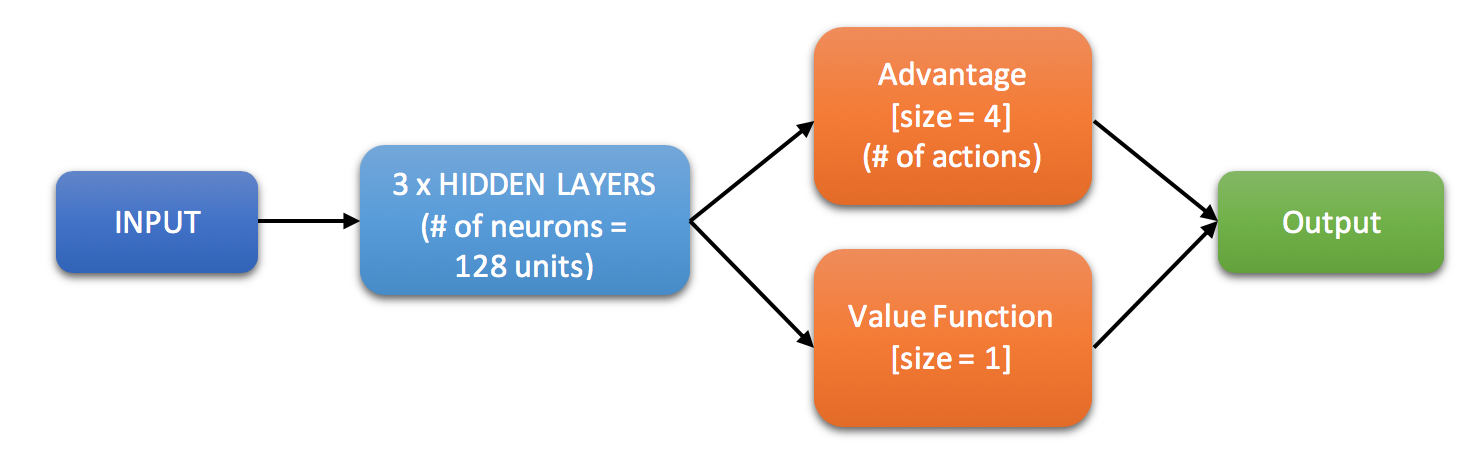
\includegraphics[width = 1\hsize]{./figures/Architecture.png} 
		\caption{Architecture of the Q-network.} % caption of the figure
		\label{fig:architecture} % a label. When we refer to this label from the text, the figure %number is included automatically
	\end{center}
\end{figure}

The hyperparameters used in training the Q-network are listed below:
\begin{center}
	\begin{tabular}{|c|c|}
	\hline
		Hyperparameter						& Value\\\hline
		Learning rate, $\alpha$				& 0.0001 \\
		Discount factor, $\gamma$		& 0.9900 \\
		Buffer size								& 500,000\\
		Soft update weights, $tau$		& 0.0010\\
		Update frequency						& 4 steps\\
		$\varepsilon_{initial}$				& 1.0000\\
		$\varepsilon_{final}$					& 0.0050\\
		$\varepsilon$- decay				& 0.9950\\\hline
	\end{tabular}
\end{center}
	
The average rewards during the training process is shown in Figure \ref{fig:rewards}. It can be observed that the agent can achieve a mean score of 13 after around 600 episodes. It took around 1800 episodes to achieve a mean score of 17.00.
	
	
\begin{figure}[H]
	\begin{center}
		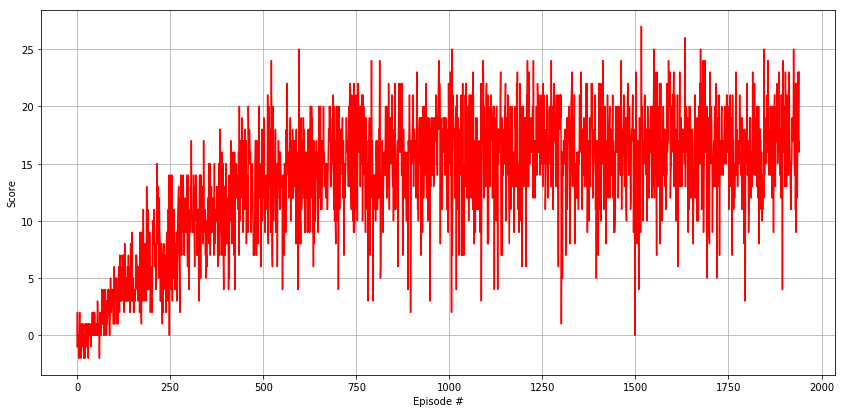
\includegraphics[width = 1\hsize]{./figures/Rewards.png} 
		\caption{Average reward vs number of episodes} % caption of the figure
		\label{fig:rewards} % a label. When we refer to this label from the text, the figure %number is included automatically
	\end{center}
\end{figure}


\section{Ideas for Future Work}
Improvements or redesign of the solution can be done in two aspects: algorithms and problem formulation. In terms of algorithms, we can potentially implement the double-Q learning, prioritized experience replay, or to depart from the estimation of action-values and opt for policy gradient methods instead. As for problem formulation, we can potentially solve the problem by learning directly from the pixels, in which we need to implement computer vision techniques to disentangle the information and patterns from each frame during game play. 	


\subsection{Choice of Algorithms}
\begin{enumerate}
	\item Double-Q Learning: Double Q-learning allows the algorithm to avoid overestimation of the Q-values as well as provide stability in the training process. In order to implement the Double Q-learning, we just need to make some small changes to the original DQN algorithhm. The DQN algorithm is based on the Q-learning algorithm which has the following update equation:
	\begin{align*}
		Q(s,a; \theta_i) \leftarrow Q(s,a; \theta_{i-1})  + \alpha\left[r + \gamma \max_{a^\prime} Q(s^\prime, a^\prime, \theta_{i-1})  - Q(s,a; \theta_i)\right].
	\end{align*}
	In Double-Q Learning, we can change the update equation to the following:
	\begin{align*}
		Q(s,a; \theta_i) \leftarrow Q(s,a; \theta_{i-1})  + \alpha\left[r + \gamma Q\left(s^\prime, \text{arg} \max_{a^\prime} Q(s^\prime, a^\prime; \theta_i); \theta_{i-1}\right)  - Q(s,a; \theta_i)\right].
	\end{align*}
	
	\item Prioritized Experience Replay: Under the current implementation, the experience replay instances are sampled uniformly. However, it is possible to quickly prioritize the different instances based on the TD error. Prioritize experience replay will shorten the training process by allowing the algorithm to focus on the instances with larger TD errors.

	\item Policy Gradient Methods: While the specific policy gradient methods have yet to be introduced, it is possible to us to solve the navigation project using policy gradient methods. Instead of having a function approximator to estimate the action-value functions, the function approximator will directly map to the appropriate function for each given state.
	
\end{enumerate}

\subsection{Learning from Pixels}
Lastly, it is possible to learn directly from the pixels of the game play. Several frames of the game play can be stacked and preprocessed in order to retain the temporal information and to reduce the input size respectively. Then preprocessed input can then be passed through a convolutional neural network to extract meaningful feature representations and to estimate the action-value function. \\

Lastly, it is important to note that the different ideas for future work are not mutually exhaustive. In fact, many of the ideas can be implemented and fine-tuned to achieve state-of-the art performance in the navigation game play.




\end{document}
%%% Local Variables: 
%%% mode: latex
%%% TeX-master: t
%%% End: 
